\documentclass[11pt,a4paper]{article}
%%%%%%%%%%%%%%%%%%%%%%%%% Credit %%%%%%%%%%%%%%%%%%%%%%%%

% template ini dibuat oleh martin.manullang@if.itera.ac.id untuk dipergunakan oleh seluruh sivitas akademik itera.

%%%%%%%%%%%%%%%%%%%%%%%%% PACKAGE starts HERE %%%%%%%%%%%%%%%%%%%%%%%%
\usepackage{graphicx}
\usepackage{caption}
\usepackage{microtype}
\usepackage{lmodern}
\captionsetup[table]{name=Tabel}
\captionsetup[figure]{name=Gambar}
\usepackage{tabulary}
\usepackage{minted}
\usepackage{amsmath}
\usepackage{fancyhdr}
\usepackage{amssymb}
\usepackage{amsthm}
\usepackage{placeins}
\usepackage{amsfonts}
\usepackage{graphicx}
\usepackage[all]{xy}
\usepackage{tikz}
\usepackage{verbatim}
\usepackage[left=2cm,right=2cm,top=3cm,bottom=2.5cm]{geometry}
\usepackage{hyperref}
\hypersetup{
    colorlinks,
    linkcolor={red!50!black},
    citecolor={blue!50!black},
    urlcolor={blue!80!black}
}
\usepackage{caption}
\usepackage{subcaption}
\usepackage{multirow}
\usepackage{psfrag}
\usepackage[T1]{fontenc}
\usepackage[scaled]{beramono}
% Enable inserting code into the document
\usepackage{listings}
\usepackage{xcolor} 
% custom color & style for listing
\definecolor{codegreen}{rgb}{0,0.6,0}
\definecolor{codegray}{rgb}{0.5,0.5,0.5}
\definecolor{codepurple}{rgb}{0.58,0,0.82}
\definecolor{backcolour}{rgb}{0.95,0.95,0.92}
\definecolor{LightGray}{gray}{0.9}
\lstdefinestyle{mystyle}{
	backgroundcolor=\color{backcolour},   
	commentstyle=\color{green},
	keywordstyle=\color{codegreen},
	numberstyle=\tiny\color{codegray},
	stringstyle=\color{codepurple},
	basicstyle=\ttfamily\footnotesize,
	breakatwhitespace=false,         
	breaklines=true,                 
	captionpos=b,                    
	keepspaces=true,                 
	numbers=left,                    
	numbersep=5pt,                  
	showspaces=false,                
	showstringspaces=false,
	showtabs=false,                  
	tabsize=2
}
\lstset{style=mystyle}
\renewcommand{\lstlistingname}{Kode}
%%%%%%%%%%%%%%%%%%%%%%%%% PACKAGE ends HERE %%%%%%%%%%%%%%%%%%%%%%%%


%%%%%%%%%%%%%%%%%%%%%%%%% Data Diri %%%%%%%%%%%%%%%%%%%%%%%%
\newcommand{\student}{\textbf{Lois Novel E Gurning (122140098)}}
\newcommand{\course}{\textbf{Sistem Teknologi Multimedia (IF25-40305)}}
\newcommand{\assignment}{\textbf{Worksheet 1: Setup Python Environment untuk Multimedia}}

%%%%%%%%%%%%%%%%%%% using theorem style %%%%%%%%%%%%%%%%%%%%
\newtheorem{thm}{Theorem}
\newtheorem{lem}[thm]{Lemma}
\newtheorem{defn}[thm]{Definition}
\newtheorem{exa}[thm]{Example}
\newtheorem{rem}[thm]{Remark}
\newtheorem{coro}[thm]{Corollary}
\newtheorem{quest}{Question}[section]
%%%%%%%%%%%%%%%%%%%%%%%%%%%%%%%%%%%%%%%%
\usepackage{lipsum}%% a garbage package you don't need except to create examples.
\usepackage{fancyhdr}
\pagestyle{fancy}
\lhead{Lois Novel E Gurning (122140098)}
\rhead{ \thepage}
\cfoot{\textbf{Worksheet 1: Setup Python Environment untuk Multimedia}}
\renewcommand{\headrulewidth}{0.4pt}
\renewcommand{\footrulewidth}{0.4pt}

%%%%%%%%%%%%%%  Shortcut for usual set of numbers  %%%%%%%%%%%

\newcommand{\N}{\mathbb{N}}
\newcommand{\Z}{\mathbb{Z}}
\newcommand{\Q}{\mathbb{Q}}
\newcommand{\R}{\mathbb{R}}
\newcommand{\C}{\mathbb{C}}
\setlength\headheight{14pt}

%%%%%%%%%%%%%%%%%%%%%%%%%%%%%%%%%%%%%%%%%%%%%%%%%%%%%%%555
\begin{document}
\thispagestyle{empty}
\begin{center}
	
\includegraphics[scale = 0.15]{Figure/ifitera-header.png}
	\vspace{0.1cm}
\end{center}
\noindent
\rule{17cm}{0.2cm}\\[0.3cm]
Nama: \student \hfill Tugas Ke: \assignment\\[0.1cm]
Mata Kuliah: \course \hfill Tanggal: \today\\
\rule{17cm}{0.05cm}
\vspace{0.1cm}



%%%%%%%%%%%%%%%%%%%%%%%%%%%%%%%%%%%%%%%%%%%%% BODY DOCUMENT %%%%%%%%%%%%%%%%%%%%%%%%%%%%%%%%%%%%%%%%%%%%%
\section{Tujuan Pembelajaran}
Setelah menyelesaikan worksheet ini, mahasiswa diharapkan mampu:
\begin{itemize}
    \item Memahami pentingnya manajemen environment Python untuk pengembangan multimedia
    \item Menginstall dan mengkonfigurasi Python environment menggunakan conda, venv, atau uv
    \item Menginstall library-library Python yang diperlukan untuk multimedia processing
    \item Memverifikasi instalasi dengan mengimpor dan menguji library multimedia
    \item Mendokumentasikan proses konfigurasi dan hasil pengujian dalam format \LaTeX
\end{itemize}

\section{Latar Belakang}
Python telah menjadi bahasa pemrograman yang sangat populer untuk multimedia processing karena memiliki ekosistem library yang sangat kaya. Namun, untuk dapat bekerja dengan multimedia secara efektif, kita perlu mengatur environment Python dengan benar dan menginstall library-library yang tepat.

Manajemen environment Python sangat penting untuk:
\begin{itemize}
    \item Menghindari konflik antar library (dependency conflict)
    \item Memastikan reproducibility dari project
    \item Memudahkan kolaborasi antar developer
    \item Memisahkan project yang berbeda dengan requirement yang berbeda
\end{itemize}

\section{Instruksi Tugas}

\subsection{Persiapan}
\textbf{Sebelum memulai, pastikan Anda telah:}
\begin{itemize}
    \item Menginstall Python 3.8 atau lebih baru di sistem Anda
    \item Memilih salah satu tool manajemen environment: \textbf{conda}, \textbf{venv}, atau \textbf{uv}
    \item Membuka terminal/command prompt
    \item Menyiapkan dokumen \LaTeX\ ini untuk dokumentasi
\end{itemize}

\subsection{Bagian 1: Membuat Environment Python}
Pilih \textbf{SALAH SATU} dari tiga opsi berikut dan ikuti langkah-langkahnya:

\subsubsection{Opsi 1: Menggunakan Conda (Direkomendasikan untuk pemula)}
Jalankan perintah berikut di terminal:

\begin{lstlisting}[language=bash, caption=Membuat environment dengan Conda]
# Membuat environment baru dengan nama 'multimedia'
conda create -n multimedia python=3.11

# Mengaktifkan environment
conda activate multimedia

# Verifikasi environment aktif
conda info --envs
\end{lstlisting}

\subsubsection{Opsi 2: Menggunakan venv (Built-in Python)}
\begin{lstlisting}[language=bash, caption=Membuat environment dengan venv]
# Membuat environment baru
python3 -m venv multimedia-env

# Mengaktifkan environment (Linux/Mac)
source multimedia-env/bin/activate

# Mengaktifkan environment (Windows)
# multimedia-env\Scripts\activate

# Verifikasi environment aktif
which python
\end{lstlisting}

\subsubsection{Opsi 3: Menggunakan uv (Modern dan cepat)}
\begin{lstlisting}[language=bash, caption=Membuat environment dengan uv]
# Install uv terlebih dahulu jika belum ada
# pip install uv

# Membuat environment baru
uv venv multimedia-uv

# Mengaktifkan environment (Linux/Mac)
source multimedia-uv/bin/activate

# Mengaktifkan environment (Windows)
# multimedia-uv\Scripts\activate

# Verifikasi environment aktif
which python
\end{lstlisting}

\textbf{Dokumentasikan di sini:}
\begin{itemize}
    \item Tool manajemen environment yang Anda pilih: \textbf{Conda}
    \item Screenshot atau copy-paste output dari perintah verifikasi environment

    \noindent
    \includegraphics[width=0.7\textwidth]{c:/Users/LENOVO/OneDrive/Pictures/Screenshots/Screenshot 2025-08-28 132750.png}
\end{itemize}

\subsection{Bagian 2: Instalasi Library Multimedia}
Setelah environment aktif, install library-library berikut:

\subsubsection{Library Audio Processing}
\begin{lstlisting}[language=bash, caption=Instalasi library audio]
# Untuk conda:
conda install -c conda-forge librosa soundfile scipy

# Untuk pip (venv/uv):
pip install librosa soundfile scipy
\end{lstlisting}

\subsubsection{Library Image Processing}
\begin{lstlisting}[language=bash, caption=Instalasi library image]
# Untuk conda:
conda install -c conda-forge opencv pillow scikit-image matplotlib

# Untuk pip (venv/uv):
pip install opencv-python pillow scikit-image matplotlib
\end{lstlisting}

\subsubsection{Library Video Processing}
\begin{lstlisting}[language=bash, caption=Instalasi library video]
# Untuk conda:
conda install -c conda-forge ffmpeg
pip install moviepy

# Untuk pip (venv/uv):
pip install moviepy
\end{lstlisting}

\subsubsection{Library General Purpose}
\begin{lstlisting}[language=bash, caption=Instalasi library umum]
# Untuk conda:
conda install numpy pandas jupyter

# Untuk pip (venv/uv):
pip install numpy pandas jupyter
\end{lstlisting}

\textbf{Dokumentasikan di sini:}
\begin{itemize}
    \item Perintah instalasi yang Anda gunakan
    \subitem 1. Audio Processing \\
    \noindent
    \hspace{1cm}\includegraphics[width=0.7\textwidth]{c:/Users/LENOVO/OneDrive/Pictures/Screenshots/Screenshot 2025-08-28 140048.png} \\
    \noindent
    \hspace{1cm}\includegraphics[width=0.7\textwidth]{c:/Users/LENOVO/OneDrive/Pictures/Screenshots/Screenshot 2025-08-28 140358.png}
    \subitem 2. Image Processing \\
    \noindent
    \hspace{1cm}\includegraphics[width=0.7\textwidth]{c:/Users/LENOVO/OneDrive/Pictures/Screenshots/Screenshot 2025-08-28 140810.png}
    \subitem 3. Video Processing \\
    \noindent
    \hspace{1cm}\includegraphics[width=0.7\textwidth]{c:/Users/LENOVO/OneDrive/Pictures/Screenshots/Screenshot 2025-08-28 141156.png} \\
    \noindent
    \hspace{1cm}\includegraphics[width=0.7\textwidth]{c:/Users/LENOVO/OneDrive/Pictures/Screenshots/Screenshot 2025-08-29 205110.png}
    \subitem 4. General Purpose \\
    \noindent
    \hspace{1cm}\includegraphics[width=0.7\textwidth]{c:/Users/LENOVO/OneDrive/Pictures/Screenshots/Screenshot 2025-08-28 141602.png}
    \item Screenshot proses instalasi atau output sukses
    \subitem 1. Audio Processing \\
    \noindent
    \hspace{1cm}\includegraphics[width=0.7\textwidth]{c:/Users/LENOVO/OneDrive/Pictures/Screenshots/Screenshot 2025-08-28 140311.png} \\
    \noindent
    \hspace{1cm}\includegraphics[width=0.7\textwidth]{c:/Users/LENOVO/OneDrive/Pictures/Screenshots/Screenshot 2025-08-28 140358.png}
    \subitem 2. Image Processing \\
    \noindent
    \hspace{1cm}\includegraphics[width=0.7\textwidth]{c:/Users/LENOVO/OneDrive/Pictures/Screenshots/Screenshot 2025-08-28 140936.png}  
    \subitem 3. Video Processing \\
    \noindent
    \hspace{1cm}\includegraphics[width=0.7\textwidth]{c:/Users/LENOVO/OneDrive/Pictures/Screenshots/Screenshot 2025-08-28 141205.png} \\
    \noindent
    \hspace{1cm}\includegraphics[width=0.7\textwidth]{c:/Users/LENOVO/OneDrive/Pictures/Screenshots/Screenshot 2025-08-28 141256.png}   
    \subitem 4. General Purpose \\
    \noindent
    \hspace{1cm}\includegraphics[width=0.7\textwidth]{c:/Users/LENOVO/OneDrive/Pictures/Screenshots/Screenshot 2025-08-28 141648.png}
    \item Daftar library yang berhasil diinstall dengan versinya \\
    \noindent
    \hspace{1cm}\includegraphics[width=0.7\textwidth]{c:/Users/LENOVO/OneDrive/Pictures/Screenshots/Screenshot 2025-08-28 141744.png} \\
    \noindent
    \hspace{1cm}\includegraphics[width=0.7\textwidth]{c:/Users/LENOVO/OneDrive/Pictures/Screenshots/Screenshot 2025-08-28 141756.png} \\
    \noindent
    \hspace{1cm}\includegraphics[width=0.7\textwidth]{c:/Users/LENOVO/OneDrive/Pictures/Screenshots/Screenshot 2025-08-28 141816.png} \\
    \noindent
    \hspace{1cm}\includegraphics[width=0.7\textwidth]{c:/Users/LENOVO/OneDrive/Pictures/Screenshots/Screenshot 2025-08-28 141832.png} \\
    \noindent
    \hspace{1cm}\includegraphics[width=0.7\textwidth]{c:/Users/LENOVO/OneDrive/Pictures/Screenshots/Screenshot 2025-08-28 141842.png}
    
\end{itemize}

\subsection{Bagian 3: Verifikasi Instalasi}
Buat file Python sederhana untuk menguji semua library yang telah diinstall:


\textbf{Jalankan script dan dokumentasikan hasilnya:}
\begin{itemize}
    \item Audio Processing
        \begin{lstlisting}[language=Python, caption={Audio Processing Sederhana dengan librosa, soundfile dan scipy}]
# Audio Processing Sederhana dengan librosa, soundfile, dan scipy
import librosa
import soundfile as sf
from scipy.signal import butter, lfilter

# Load audio file
audio_path = 'mulmedtesting.wav'  # Ganti dengan path file audio Anda
y, sr = librosa.load(audio_path, sr=None)

# Simpan ulang audio menggunakan soundfile
sf.write('output_audio.wav', y, sr)

# Filter Butterworth (lowpass)
def butter_lowpass(cutoff, fs, order=5):
    nyq = 0.5 * fs
    normal_cutoff = cutoff / nyq
    b, a = butter(order, normal_cutoff, btype='low', analog=False)
    return b, a

def lowpass_filter(data, cutoff, fs, order=5):
    b, a = butter_lowpass(cutoff, fs, order=order)
    y = lfilter(b, a, data)
    return y

# Terapkan filter lowpass pada audio
filtered_audio = lowpass_filter(y, cutoff=4000, fs=sr, order=6)

# Simpan hasil audio yang sudah difilter
sf.write('filtered_audio.wav', filtered_audio, sr)

print('Audio processing selesai!')
        \end{lstlisting}
        \begin{flushleft}
            \includegraphics[width=0.35\textwidth]{c:/Users/LENOVO/OneDrive/Pictures/Screenshots/Screenshot 2025-08-29 212227.png}
        \end{flushleft}
        \begin{flushleft}
            \includegraphics[width=0.35\textwidth]{c:/Users/LENOVO/OneDrive/Pictures/Screenshots/Screenshot 2025-08-29 212757.png}
        \end{flushleft}
    \item Image Processing
        \begin{lstlisting}[language=Python, caption={Image Processing Sederhana dengan OpenCV, Pillow, scikit-image, dan matplotlib}]
# Image Processing Sederhana dengan OpenCV, Pillow, scikit-image, dan matplotlib
import cv2
from PIL import Image
from skimage import filters, color
import matplotlib.pyplot as plt

# Load gambar menggunakan OpenCV
img_cv = cv2.imread('gambartesting.jpg')  # Ganti dengan path file gambar Anda
img_cv_rgb = cv2.cvtColor(img_cv, cv2.COLOR_BGR2RGB)

# Load gambar menggunakan Pillow
img_pil = Image.open('gambartesting.jpg')

# Konversi ke grayscale dengan scikit-image
img_gray = color.rgb2gray(img_cv_rgb)

# Deteksi tepi dengan Sobel (scikit-image)
edges = filters.sobel(img_gray)

# Tampilkan hasil dengan matplotlib
fig, axes = plt.subplots(1, 3, figsize=(12, 4))
axes[0].imshow(img_cv_rgb)
axes[0].set_title('Original (OpenCV)')
axes[1].imshow(img_pil)
axes[1].set_title('Original (Pillow)')
axes[2].imshow(edges, cmap='gray')
axes[2].set_title('Sobel Edges (scikit-image)')
for ax in axes:
    ax.axis('off')
plt.tight_layout()
plt.show()
        \end{lstlisting}
        \begin{flushleft}
            \includegraphics[width=0.7\textwidth]{c:/Users/LENOVO/OneDrive/Pictures/Screenshots/Screenshot 2025-08-29 213720.png}
        \end{flushleft}
    \item Video Processing
        \begin{lstlisting}[language=Python, caption={Video Processing Sederhana dengan ffmpeg dan moviepy}]
# Video Processing Sederhana dengan ffmpeg dan moviepy
import moviepy
from moviepy.editor import VideoFileClip, vfx
import subprocess

# Path video input dan output
input_video = 'videotesting.mp4'  # Ganti dengan path file video Anda
output_video = 'output_video.mp4'

# Contoh: Ekstrak audio dari video menggunakan ffmpeg
subprocess.run(['ffmpeg', '-i', input_video, '-q:a', '0', '-map', 'a', 'extracted_audio.mp3'])

# Contoh: Potong video 0-5 detik dan ubah ke grayscale dengan moviepy
clip = VideoFileClip(input_video).subclip(0, 5)
gray_clip = clip.fx(vfx.blackwhite)
gray_clip.write_videofile(output_video)

print('Video processing selesai!')
        \end{lstlisting}
            \begin{flushleft}
                \includegraphics[width=0.7\textwidth]{c:/Users/LENOVO/OneDrive/Pictures/Screenshots/Screenshot 2025-08-29 213856.png}
            \end{flushleft}
            \begin{flushleft}
                \includegraphics[width=0.7\textwidth]{c:/Users/LENOVO/OneDrive/Pictures/Screenshots/Screenshot 2025-08-29 213915.png}          \end{flushleft}
            \item General Purpose
        \begin{lstlisting}[language=Python, caption={General Purpose Test dengan numpy, pandas, dan jupyter}]
# Testing library numpy, pandas, dan jupyter
import numpy as np
import pandas as pd
from IPython.display import display, Markdown

# Numpy: operasi array sederhana
arr = np.array([1, 2, 3, 4, 5])
arr_squared = arr ** 2
print('Array:', arr)
print('Array kuadrat:', arr_squared)

# Pandas: membuat dan menampilkan DataFrame sederhana
df = pd.DataFrame({'Angka': arr, 'Kuadrat': arr_squared})
display(df)

# Jupyter: menampilkan markdown dari kode
display(Markdown('**Tes berhasil! Semua library dapat digunakan.**'))
        \end{lstlisting}
        \begin{flushleft}
            \includegraphics[width=0.6\textwidth]{c:/Users/LENOVO/OneDrive/Pictures/Screenshots/Screenshot 2025-08-29 214448.png}
        \end{flushleft}
\end{itemize}

\subsection{Bagian 4: Simple Test dengan Sample Code}
Buat dan jalankan contoh sederhana untuk setiap kategori multimedia:

\subsubsection{Test Audio Processing}
\begin{lstlisting}[language=Python, caption=Test audio processing sederhana]
import numpy as np
import matplotlib.pyplot as plt

# Generate simple sine wave
duration = 2  # seconds
sample_rate = 44100
frequency = 440  # A4 note

t = np.linspace(0, duration, int(sample_rate * duration))
audio_signal = np.sin(2 * np.pi * frequency * t)

# Plot waveform
plt.figure(figsize=(10, 4))
plt.plot(t[:1000], audio_signal[:1000])  # Plot first 1000 samples
plt.title('Sine Wave (440 Hz)')
plt.xlabel('Time (s)')
plt.ylabel('Amplitude')
plt.grid(True)
plt.savefig('sine_wave_test.png', dpi=150, bbox_inches='tight')
plt.show()

print(f"Generated {duration}s sine wave at {frequency}Hz")
print(f"Sample rate: {sample_rate}Hz")
print(f"Total samples: {len(audio_signal)}")
\end{lstlisting}

\subsubsection{Test Image Processing}
\begin{lstlisting}[language=Python, caption=Test image processing sederhana]
import numpy as np
import matplotlib.pyplot as plt
from PIL import Image

# Create a simple test image
width, height = 400, 300
image = np.zeros((height, width, 3), dtype=np.uint8)

# Add some patterns
image[:, :width//3, 0] = 255  # Red section
image[:, width//3:2*width//3, 1] = 255  # Green section
image[:, 2*width//3:, 2] = 255  # Blue section

# Add a white circle in the center
center_x, center_y = width//2, height//2
radius = 50
Y, X = np.ogrid[:height, :width]
mask = (X - center_x)**2 + (Y - center_y)**2 <= radius**2
image[mask] = [255, 255, 255]

# Display and save
plt.figure(figsize=(8, 6))
plt.imshow(image)
plt.title('Test Image with RGB Stripes and White Circle')
plt.axis('off')
plt.savefig('test_image.png', dpi=150, bbox_inches='tight')
plt.show()

print(f"Created test image: {width}x{height} pixels")
print(f"Image shape: {image.shape}")
print(f"Image dtype: {image.dtype}")
\end{lstlisting}

\textbf{Dokumentasikan hasil eksekusi:}
\begin{itemize}
    \item Screenshot output dari kedua script di atas
    \subitem 1. Test Audio Processing
    \begin{flushleft}
        \includegraphics[width=0.7\textwidth]{c:/Users/LENOVO/OneDrive/Pictures/Screenshots/Screenshot 2025-08-29 215144.png}
    \end{flushleft}
    \subitem 2. Test Image Processing
        \begin{flushleft}
            \includegraphics[width=0.7\textwidth]{c:/Users/LENOVO/OneDrive/Pictures/Screenshots/Screenshot 2025-08-29 215154.png}
    \end{flushleft}
    \item Gambar yang dihasilkan (sine\_wave\_test.png dan test\_image.png)
    \subitem 1. Sine Wave
        \begin{flushleft}
            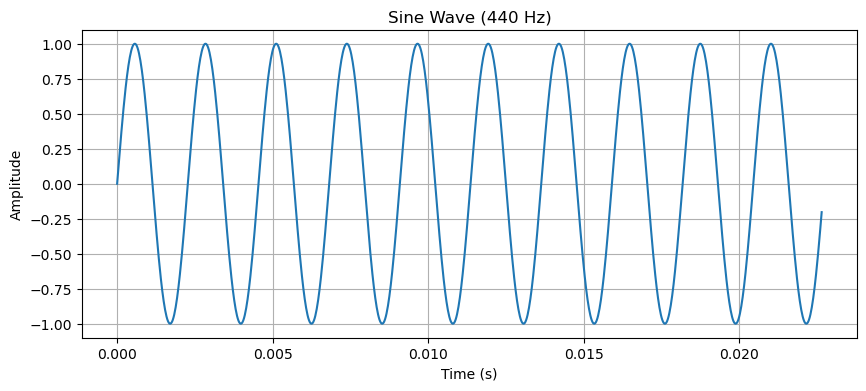
\includegraphics[width=0.7\textwidth]{d:/Download/Semester 7/Mulmed/output.png}
    \end{flushleft}
    \subitem 2. Test Image
        \begin{flushleft}
            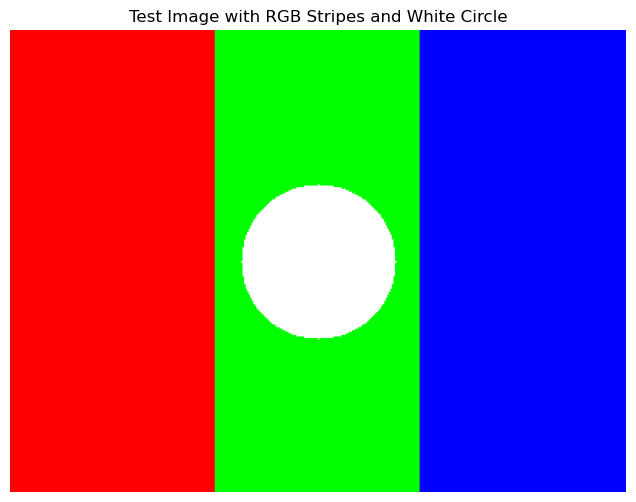
\includegraphics[width=0.7\textwidth]{d:/Download/Semester 7/Mulmed/output2.png}
    \end{flushleft}
    \item Error message jika ada dan cara mengatasinya \\
    \textit{[Tidak ada]}
\end{itemize}

\section{Bagian Laporan}

\subsection{Output Verifikasi Instalasi}
\textbf{Copy-paste output lengkap dari script \texttt{test\_multimedia.py} di sini:}

\begin{lstlisting}[caption=Output verifikasi instalasi]
# Audio Processing
Generated 2s sine wave at 440 Hz
Sample rate: 44100 Hz
Total samples: 88200

# Image Processing
Created test image: 400x300 pixels
Image shape: (300, 400, 3)
Image dtype: uint8
\end{lstlisting}

\subsection{Screenshot Hasil Test}
\textbf{Sisipkan screenshot atau gambar hasil dari:}
\begin{itemize}
    \item Terminal/command prompt yang menunjukkan environment aktif
    \begin{flushleft}
        \includegraphics[width=0.7\textwidth]{c:/Users/LENOVO/OneDrive/Pictures/Screenshots/Screenshot 2025-08-28 132750.png}
    \end{flushleft}
    \item Output dari script test audio (sine wave plot)
    \begin{flushleft}
        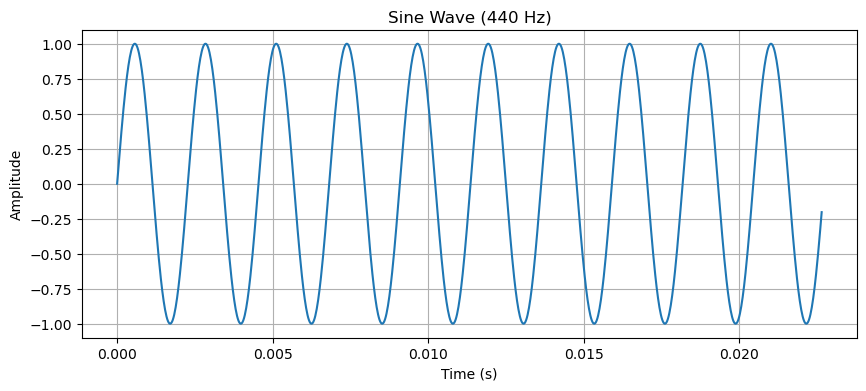
\includegraphics[width=0.7\textwidth]{d:/Download/Semester 7/Mulmed/output.png}
    \end{flushleft}
    \item Output dari script test image (RGB stripes dengan circle)
    \begin{flushleft}
        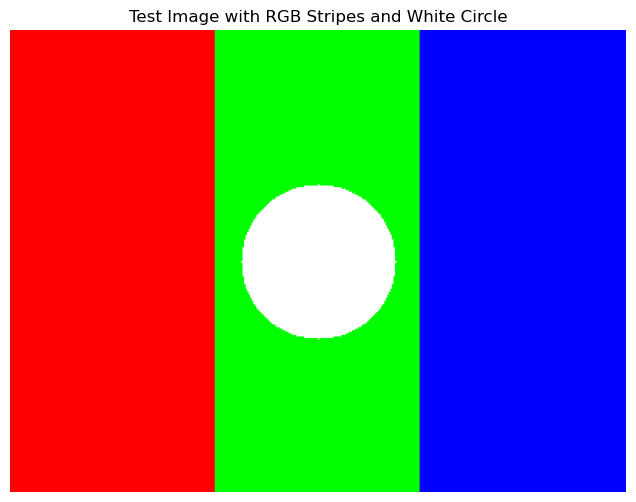
\includegraphics[width=0.7\textwidth]{d:/Download/Semester 7/Mulmed/output2.png}
    \end{flushleft}
\end{itemize}

\subsection{Analisis dan Refleksi}
\textbf{Jawab pertanyaan berikut:}

\begin{enumerate}
    \item \textbf{Mengapa penting menggunakan environment terpisah untuk project multimedia?}
    
    \textit{[Menggunakan environment terpisah untuk project multimedia sangat penting karena dapat mengisolasi dependency agar tidak terjadi konflik versi antar library, menjaga stabilitas project meskipun ada update library di project lain, serta memudahkan reproduksi melalui file environment.yml sehingga konfigurasi bisa dipindahkan atau dibagikan ke tim dengan konsisten. Selain itu, environment terpisah memungkinkan instalasi backend eksternal seperti ffmpeg atau libsndfile tanpa mengganggu project lain, meningkatkan performa serta kompatibilitas, dan memberi ruang aman untuk bereksperimen dengan berbagai versi library tanpa risiko merusak environment global.]}
    
    \item \textbf{Apa perbedaan utama antara conda, venv, dan uv? Mengapa Anda memilih tool yang Anda gunakan?}
    
    \textit{[Perbedaan utama antara conda, venv, dan uv terletak pada cakupan serta kecepatan manajemen environment. Conda adalah package dan environment manager lintas bahasa yang dapat mengelola library Python maupun non-Python, sehingga cocok untuk project ilmiah dan multimedia yang kompleks. Venv adalah tool bawaan Python yang lebih ringan, hanya membuat virtual environment khusus Python tanpa manajemen dependency eksternal, sehingga cocok untuk project sederhana atau web development. Uv adalah tool baru yang sangat cepat untuk manajemen dependency dan environment Python, fokus pada efisiensi instalasi serta reproducibility modern.
    Saya memilih conda karena conda tidak hanya mengelola environment Python, tetapi juga mampu mengatur dependency lintas bahasa dan library eksternal yang sering dibutuhkan pada project kompleks. Selain itu, conda memudahkan reproduksi environment melalui file environment.yml, mendukung berbagai channel seperti conda-forge untuk ketersediaan paket yang luas, dan memungkinkan pengelolaan environment yang terisolasi agar project tetap konsisten serta tidak saling mengganggu.]}
    
    \item \textbf{Library mana yang paling sulit diinstall dan mengapa?}
    
    \textit{[Sejauh saya mencoba, tidak ada kesulitan yang saya alami dalam menginstall library-library tersebut karena seluruh dependency dapat terpasang dengan baik melalui conda maupun pip, sehingga proses instalasi berjalan lancar tanpa konflik versi maupun error tambahan.]}
    
    \item \textbf{Bagaimana cara mengatasi masalah dependency conflict jika terjadi?}
    
    \textit{[Masalah dependency conflict dapat diatasi dengan membuat environment terpisah untuk setiap project agar dependency tidak saling mengganggu, menggunakan channel yang konsisten seperti conda-forge untuk menghindari perbedaan sumber paket, serta menetapkan versi library secara eksplisit agar tidak terjadi pertentangan versi. Selain itu, instalasi sebaiknya dilakukan berurutan, yaitu memasang library utama melalui conda terlebih dahulu lalu melengkapi dengan pip hanya jika paket tidak tersedia di conda.]}
    
    \item \textbf{Jelaskan fungsi dari masing-masing library yang berhasil Anda install!}
    
    \textit{
        \\1. Librosa → Library Python untuk analisis dan pemrosesan sinyal audio, misalnya ekstraksi fitur (MFCC, chroma, spectral contrast) dalam penelitian musik, suara, atau speech. \\
        2. Soundfile → Digunakan untuk membaca dan menulis file audio (WAV, FLAC, OGG, dsb.) dengan performa tinggi menggunakan backend libsndfile. \\
        3. Scipy → Library ilmiah yang menyediakan fungsi matematika, optimisasi, sinyal, statistika, hingga pemrosesan data numerik tingkat lanjut. \\
        4. OpenCV → Framework computer vision populer untuk pengolahan citra dan video, seperti deteksi objek, face recognition, filtering, dan transformasi citra. \\
        5. Pillow (PIL Fork) → Library manipulasi gambar (image processing) yang mendukung banyak format file (JPEG, PNG, BMP, dsb.), misalnya resize, crop, filter, dan konversi. \\
        6. Scikit-image → Khusus untuk pengolahan citra berbasis scientific computing, menyediakan fungsi segmentasi, filtering, feature extraction, dan image enhancement. \\
        7. Matplotlib → Library visualisasi data untuk membuat grafik 2D/3D, scatter plot, histogram, hingga visualisasi sinyal atau gambar. \\
        8. FFmpeg → Software open-source untuk decoding, encoding, konversi format, serta manipulasi audio dan video (dipanggil lewat command line maupun binding Python). \\
        9. Moviepy → Library editing video berbasis Python yang memungkinkan pemotongan, penggabungan, penambahan efek, ekstraksi audio, hingga render video menggunakan backend FFmpeg. \\
        10. NumPy → Dasar scientific computing di Python yang menyediakan array multidimensi dan operasi matematika/linear algebra berkecepatan tinggi. \\
        11. Pandas → Library manajemen dan analisis data berbasis DataFrame dengan kemampuan powerful untuk manipulasi, cleaning, dan analisis data tabular. \\
        12. Jupyter → Platform interaktif berbasis notebook yang memungkinkan menjalankan kode Python, visualisasi, dan dokumentasi dalam satu dokumen.
    }
\end{enumerate}

\subsection{Troubleshooting}
\textbf{Dokumentasikan masalah yang Anda hadapi (jika ada) dan cara mengatasinya:}

\textit{[Tidak ada]}

\section{Export Environment untuk Reproduksi}
Sebagai langkah terakhir, export environment Anda agar dapat direproduksi:

\subsection{Untuk Conda}
\begin{lstlisting}[language=bash, caption=Export conda environment]
conda env export > environment.yml
\end{lstlisting}

\subsection{Untuk venv/uv}
\begin{lstlisting}[language=bash, caption=Export pip requirements]
pip freeze > requirements.txt
\end{lstlisting}

\textbf{Copy-paste isi file environment.yml atau requirements.txt di sini:}

\begin{lstlisting}[caption=Environment/Requirements file]
[name: multimedia
channels:
  - defaults
  - conda-forge
  - https://repo.anaconda.com/pkgs/main
  - https://repo.anaconda.com/pkgs/r
  - https://repo.anaconda.com/pkgs/msys2
dependencies:
  - _libavif_api=1.3.0=h57928b3_2
  - anyio=4.7.0=py311haa95532_0
  - aom=3.9.1=he0c23c2_0
  - argon2-cffi=21.3.0=pyhd3eb1b0_0
  - argon2-cffi-bindings=21.2.0=py311h827c3e9_1
  - asttokens=3.0.0=py311haa95532_0
  - async-lru=2.0.4=py311haa95532_0
  - attrs=24.3.0=py311haa95532_0
  - audioread=3.0.1=py311h1ea47a8_2
  - babel=2.16.0=py311haa95532_0
  - beautifulsoup4=4.13.4=py311haa95532_0
  - blas=1.0=mkl
  - bleach=6.2.0=py311haa95532_0
  - bottleneck=1.4.2=py311h57dcf0c_0
  - brotli=1.1.0=h2466b09_3
  - brotli-bin=1.1.0=h2466b09_3
  - brotli-python=1.1.0=py311hda3d55a_3
  - bzip2=1.0.8=h2bbff1b_6
  - ca-certificates=2025.8.3=h4c7d964_0
  - cairo=1.18.4=he9e932c_0
  - certifi=2025.8.3=pyhd8ed1ab_0
  - cffi=1.17.1=py311he736701_0
  - charset-normalizer=3.4.3=pyhd8ed1ab_0
  - colorama=0.4.6=py311haa95532_0
  - comm=0.2.1=py311haa95532_0
  - contourpy=1.3.3=py311h3fd045d_1
  - cycler=0.12.1=pyhd8ed1ab_1
  - dav1d=1.2.1=hcfcfb64_0
  - debugpy=1.8.11=py311h5da7b33_0
  - decorator=5.2.1=pyhd8ed1ab_0
  - defusedxml=0.7.1=pyhd3eb1b0_0
  - eigen=3.4.0=h91493d7_0
  - executing=0.8.3=pyhd3eb1b0_0
  - expat=2.7.1=h8ddb27b_0
  - ffmpeg=4.3.1=ha925a31_0
  - fontconfig=2.14.1=hb33846d_3
  - fonttools=4.59.2=py311h3f79411_0
  - freeglut=3.4.0=h8a1e904_1
  - freetype=2.13.3=h0620614_0
  - fribidi=1.0.10=h8d14728_0
  - gflags=2.2.2=he0c23c2_1005
  - glog=0.5.0=h4797de2_0
  - graphite2=1.3.14=hac47afa_2
  - gst-plugins-base=1.24.12=h91a6125_1
  - gstreamer=1.24.12=hfb93a4f_1
  - gstreamer-orc=0.4.41=h1f81b68_0
  - h11=0.16.0=py311haa95532_0
  - h2=4.2.0=pyhd8ed1ab_0
  - harfbuzz=10.2.0=he2f9f60_1
  - hdf5=1.14.5=ha36df97_2
  - hpack=4.1.0=pyhd8ed1ab_0
  - httpcore=1.0.9=py311haa95532_0
  - httpx=0.28.1=py311haa95532_0
  - hyperframe=6.1.0=pyhd8ed1ab_0
  - icc_rt=2022.1.0=h6049295_2
  - icu=73.2=h63175ca_0
  - idna=3.10=pyhd8ed1ab_1
  - imageio=2.37.0=pyhfb79c49_0
  - importlib-metadata=8.7.0=pyhe01879c_1
  - intel-openmp=2025.0.0=haa95532_1164
  - ipykernel=6.29.5=py311haa95532_1
  - ipython=9.1.0=py311haa95532_0
  - ipython_pygments_lexers=1.1.1=py311haa95532_0
  - ipywidgets=8.1.5=py311haa95532_0
  - jedi=0.19.2=py311haa95532_0
  - jinja2=3.1.6=py311haa95532_0
  - joblib=1.5.2=pyhd8ed1ab_0
  - jpeg=9e=hcfcfb64_3
  - json5=0.9.25=py311haa95532_0
  - jsonschema=4.25.0=py311haa95532_0
  - jsonschema-specifications=2023.7.1=py311haa95532_0
  - jupyter=1.1.1=py311haa95532_0
  - jupyter-lsp=2.2.5=py311haa95532_0
  - jupyter_client=8.6.3=py311haa95532_0
  - jupyter_console=6.6.3=py311haa95532_0
  - jupyter_core=5.8.1=py311haa95532_0
  - jupyter_events=0.12.0=py311haa95532_0
  - jupyter_server=2.16.0=py311haa95532_0
  - jupyter_server_terminals=0.5.3=py311haa95532_0
  - jupyterlab=4.4.4=py311haa95532_0
  - jupyterlab_pygments=0.3.0=py311haa95532_0
  - jupyterlab_server=2.27.3=py311haa95532_0
  - jupyterlab_widgets=3.0.15=py311haa95532_0
  - kiwisolver=1.4.9=py311h275cad7_0
  - lame=3.100=hcfcfb64_1003
  - lazy-loader=0.4=pyhd8ed1ab_2
  - lazy_loader=0.4=pyhd8ed1ab_2
  - lcms2=2.16=h62be587_1
  - lerc=4.0.0=h6470a55_1
  - libabseil=20250127.0=cxx17_h4eb7d71_0
  - libavif=1.3.0=he916da2_2
  - libavif16=1.3.0=he916da2_2
  - libbrotlicommon=1.1.0=h2466b09_3
  - libbrotlidec=1.1.0=h2466b09_3
  - libbrotlienc=1.1.0=h2466b09_3
  - libclang13=14.0.6=default_h8e68704_2
  - libdeflate=1.22=h2466b09_0
  - libffi=3.4.4=hd77b12b_1
  - libflac=1.4.3=h63175ca_0
  - libglib=2.84.2=h405b238_0
  - libhwloc=2.12.1=default_h88281d1_1000
  - libiconv=1.18=hc1393d2_2
  - libkrb5=1.21.3=h885b0b7_4
  - libogg=1.3.5=h2466b09_1
  - libopus=1.5.2=h2466b09_0
  - libpng=1.6.39=h8cc25b3_0
  - libpq=17.4=h4a159e6_2
  - libprotobuf=5.29.3=h65a231f_1
  - librosa=0.11.0=pyhd8ed1ab_0
  - libsndfile=1.2.2=h81429f1_1
  - libsodium=1.0.18=h62dcd97_0
  - libtiff=4.7.0=h404307b_0
  - libvorbis=1.3.7=h5112557_2
  - libwebp-base=1.6.0=h4d5522a_0
  - libwinpthread=12.0.0.r4.gg4f2fc60ca=h57928b3_9
  - libxml2=2.13.8=h866ff63_0
  - libxslt=1.1.43=h25c3957_0
  - llvm-openmp=20.1.8=h29ce207_0
  - llvmlite=0.44.0=py311h8b1c7eb_1
  - lz4-c=1.9.4=hcfcfb64_0
  - markupsafe=3.0.2=py311h827c3e9_0
  - matplotlib=3.10.1=py311h1ea47a8_0
  - matplotlib-base=3.10.1=py311h8f1b1e4_0
  - matplotlib-inline=0.1.6=py311haa95532_0
  - minizip=4.0.3=hb68bac4_0
  - mistune=3.1.2=py311haa95532_0
  - mkl=2025.0.0=h5da7b33_930
  - mkl-service=2.4.0=py311h827c3e9_3
  - mkl_fft=1.3.11=py311h5810407_1
  - mkl_random=1.2.8=py311h8683371_1
  - moviepy=1.0.3=pyhd8ed1ab_1
  - mpg123=1.32.9=h01009b0_0
  - msgpack-python=1.1.1=py311h3257749_0
  - munkres=1.1.4=pyhd8ed1ab_1
  - nbclient=0.10.2=py311haa95532_0
  - nbconvert=7.16.6=py311haa95532_0
  - nbconvert-core=7.16.6=py311haa95532_0
  - nbconvert-pandoc=7.16.6=py311haa95532_0
  - nbformat=5.10.4=py311haa95532_0
  - nest-asyncio=1.6.0=py311haa95532_0
  - networkx=3.5=pyhe01879c_0
  - notebook=7.4.4=py311haa95532_0
  - notebook-shim=0.2.4=py311haa95532_0
  - numba=0.61.2=py311h7afb941_1
  - numexpr=2.11.0=py311ha02bb35_1
  - numpy=2.2.5=py311h12f7302_1
  - numpy-base=2.2.5=py311he4e2855_1
  - opencv=4.10.0=py311h28596fa_7
  - openjpeg=2.5.2=h9b5d1b5_1
  - openssl=3.5.2=h725018a_0
  - overrides=7.4.0=py311haa95532_0
  - packaging=25.0=pyh29332c3_1
  - pandas=2.3.1=py311h885b0b7_0
  - pandoc=2.12=haa95532_3
  - pandocfilters=1.5.0=pyhd3eb1b0_0
  - parso=0.8.4=py311haa95532_0
  - pcre2=10.42=h0ff8eda_1
  - pillow=11.3.0=py311hb328d1f_0
  - pip=25.1=pyhc872135_2
  - pixman=0.46.4=h5112557_1
  - platformdirs=4.4.0=pyhcf101f3_0
  - pooch=1.8.2=pyhd8ed1ab_3
  - prometheus_client=0.21.1=py311haa95532_0
  - prompt-toolkit=3.0.43=py311haa95532_0
  - prompt_toolkit=3.0.43=hd3eb1b0_0
  - psutil=5.9.0=py311h827c3e9_1
  - pure_eval=0.2.2=pyhd3eb1b0_0
  - pycparser=2.22=pyh29332c3_1
  - pygments=2.19.1=py311haa95532_0
  - pyparsing=3.2.3=pyhe01879c_2
  - pyqt=6.7.1=py311h378bd72_2
  - pyqt6-sip=13.9.1=py311h02ab6af_2
  - pyside6=6.7.3=py311h28b127d_1
  - pysocks=1.7.1=pyh09c184e_7
  - pysoundfile=0.13.1=pyhd8ed1ab_0
  - python=3.11.13=h981015d_0
  - python-dateutil=2.9.0.post0=pyhe01879c_2
  - python-fastjsonschema=2.20.0=py311haa95532_0
  - python-json-logger=3.2.1=py311haa95532_0
  - python-tzdata=2025.2=pyhd3eb1b0_0
  - python_abi=3.11=2_cp311
  - pytz=2025.2=py311haa95532_0
  - pywavelets=1.9.0=py311h17033d2_0
  - pywin32=311=py311h885b0b7_0
  - pywinpty=2.0.15=py311h72d21ff_0
  - pyyaml=6.0.2=py311h827c3e9_0
  - pyzmq=26.2.0=py311h5da7b33_0
  - qhull=2020.2=hc790b64_5
  - qtbase=6.7.3=hd088775_4
  - qtconsole=5.6.1=py311haa95532_1
  - qtdeclarative=6.7.3=h885b0b7_1
  - qtpy=2.4.1=py311haa95532_0
  - qtshadertools=6.7.3=h885b0b7_1
  - qtsvg=6.7.3=h9d4b640_1
  - qttools=6.7.3=hcb596f7_1
  - qtwebchannel=6.7.3=h885b0b7_1
  - qtwebengine=6.7.3=h3869032_1
  - qtwebsockets=6.7.3=h885b0b7_1
  - rav1e=0.7.1=ha073cba_3
  - referencing=0.30.2=py311haa95532_0
  - requests=2.32.5=pyhd8ed1ab_0
  - rfc3339-validator=0.1.4=py311haa95532_0
  - rfc3986-validator=0.1.1=py311haa95532_0
  - rpds-py=0.22.3=py311h636fa0f_0
  - scikit-image=0.25.2=py311hcf9f919_0
  - scikit-learn=1.7.1=py311h8a15ebc_0
  - scipy=1.16.0=py311h3690d35_1
  - send2trash=1.8.2=py311haa95532_1
  - setuptools=72.1.0=py311haa95532_0
  - sip=6.10.0=py311h5da7b33_0
  - six=1.17.0=pyhe01879c_1
  - sniffio=1.3.0=py311haa95532_0
  - soupsieve=2.5=py311haa95532_0
  - soxr=0.1.3=hcfcfb64_3
  - soxr-python=0.5.0.post1=py311hda3d55a_1
  - sqlite=3.50.2=hda9a48d_1
  - stack_data=0.2.0=pyhd3eb1b0_0
  - standard-aifc=3.13.0=py311h1ea47a8_2
  - standard-sunau=3.13.0=py311h1ea47a8_2
  - svt-av1=3.1.2=hac47afa_0
  - tbb=2022.0.0=h214f63a_0
  - tbb-devel=2022.0.0=h214f63a_0
  - terminado=0.17.1=py311haa95532_0
  - threadpoolctl=3.6.0=pyhecae5ae_0
  - tifffile=2025.2.18=py311haa95532_0
  - tinycss2=1.4.0=py311haa95532_0
  - tk=8.6.15=hf199647_0
  - tornado=6.5.2=py311h3485c13_0
  - traitlets=5.14.3=py311haa95532_0
  - typing-extensions=4.15.0=py311haa95532_0
  - typing_extensions=4.15.0=py311haa95532_0
  - tzdata=2025b=h04d1e81_0
  - ucrt=10.0.22621.0=haa95532_0
  - unicodedata2=16.0.0=py311he736701_0
  - urllib3=2.5.0=pyhd8ed1ab_0
  - vc=14.3=h2df5915_10
  - vc14_runtime=14.44.35208=h4927774_10
  - vs2015_runtime=14.44.35208=ha6b5a95_10
  - wcwidth=0.2.13=py311haa95532_0
  - webencodings=0.5.1=py311haa95532_1
  - websocket-client=1.8.0=py311haa95532_0
  - wheel=0.45.1=py311haa95532_0
  - widgetsnbextension=4.0.13=py311haa95532_0
  - win_inet_pton=1.1.0=pyh7428d3b_8
  - winpty=0.4.3=4
  - xz=5.6.4=h4754444_1
  - yaml=0.2.5=he774522_0
  - zeromq=4.3.5=hd77b12b_0
  - zipp=3.23.0=pyhd8ed1ab_0
  - zlib=1.2.13=h8cc25b3_1
  - zstandard=0.23.0=py311h3485c13_3
  - zstd=1.5.6=h8880b57_0
  - pip:
      - imageio-ffmpeg==0.6.0
      - proglog==0.1.12
      - python-dotenv==1.1.1
      - tqdm==4.67.1
prefix: D:\Miniconda\envs\multimedia
]
\end{lstlisting}

\section{Kesimpulan}
\textbf{Tuliskan kesimpulan Anda mengenai:}
\begin{itemize}
    \item Pengalaman setup Python environment untuk multimedia
    \item Persiapan untuk project multimedia selanjutnya
    \item Saran untuk mahasiswa lain yang akan melakukan setup serupa
\end{itemize}

\textit{\\1. Setup environment berjalan lancar dengan bantuan conda, yang mempermudah instalasi library multimedia seperti librosa, soundfile, opencv, moviepy, dan ffmpeg tanpa masalah dependency. \\
}
\textit{\\2. Environment yang sudah terstruktur rapi dan terdokumentasi dalam file environment.yml dapat langsung digunakan kembali atau direproduksi, sehingga mempercepat persiapan project multimedia berikutnya. \\
}
\textit{\\3. Saran untuk mahasiswa lain yang akan melakukan setup serupa adalah agar selalu menggunakan environment terpisah di conda sehingga terhindar dari konflik versi antar library. Selain itu, sebaiknya prioritaskan instalasi library melalui channel conda-forge karena lebih stabil dan lengkap, kemudian gunakan pip hanya jika library yang dibutuhkan tidak tersedia di conda. Terakhir, dokumentasikan environment menggunakan perintah conda env export agar konfigurasi yang sudah dibuat dapat dengan mudah dibagikan atau digunakan ulang di perangkat lain sehingga proses setup menjadi lebih efisien dan konsisten.
}

\section{Referensi}
\href{https://chatgpt.com/share/68b1c584-4bec-8003-93e8-a874f66dc8d0}{Link Referensi}

\end{document}